% !TeX spellcheck = en_US

\section{Motivation}
Motivation:Biologische Proben sowohl unterm Licht- als auch Elektronenmikroskob anschauen

\section{State-of-the-art}

\subsection{Methods for getting rid of ice xD}

There are four passive anti-frosing strategies: Inhibition of ice nucleation is archieved by using surface inherent properties and heating to prevent ice crystals to form. Retardation of frosting removes water over time to prevent icing on the surface with water repellent properties such as the lotus effect. Mitigation of frost accumulation prevents already formed ice droplets to further accumulate and forming an ice layer. Last a reduction of ice adhesion so ice needs less force to detach of a surface even until ice droplets are not able to attach to a surface, detaching themself with the force of gravity \cite{Yang.2021}. 

\subsection{PDMS application (in z.b. der Flugindustrie)}

\subsection{Assemblies used at cryogenic temperatures}

In advance, two specialized assemblies designed before this master thesis are used throughout the master thesis. These tools created for partially different purposes.

First a bath for sample preparation is used. This Bath is filled with liquid nitrogen for cooling. The second floor is elevated of the bath floor, serving as base plate for other smaller assembly and as work station with dents for other tools and easier use for samples. In normal use, the base plate is submerged in liquid nitrogen. Fixed on the base plate and elevated over the liquid nitrogen, small tanks for other liquids are installed, which can be temperature controlled. Then also elevated a harbor for an harbor-shuttle system is installed for a fast and precise transport of samples.

The Shuttles are also used in cryo light microscopes. The Microscope used for cryotemperatures have an additional box installed, routing Cold nitrogen gas underneath a harbor, where the sample is placed. Heaters are placed around the box and under the harbor to archieve a constant temperature. On top of the Harbor, warm Nitrogen is blown so no ice is forming inside the optical path. 

Second, an assembly to lift samples at cryogenic temperatures, also called finger, is used. The finger has two main parts: A metal rod with a slightly pointed tip (Fig. \ref{fig:querschnittfinger}). Near the tip, the rod is also temperature controlled with a temperature sensor and a heater. On the tip, a glue like HFE can be used to glue onto the sample. The second main part is a 3D printed part, containing the outer shell and routing of the cold gaseous nitrogen. The nitrogen is first flowing inside and around the metal bar for cooling. then, the Gas is flowing through an outer mantle for additional cooling and out on top.


\begin{figure}[hbt!]
	\centering
	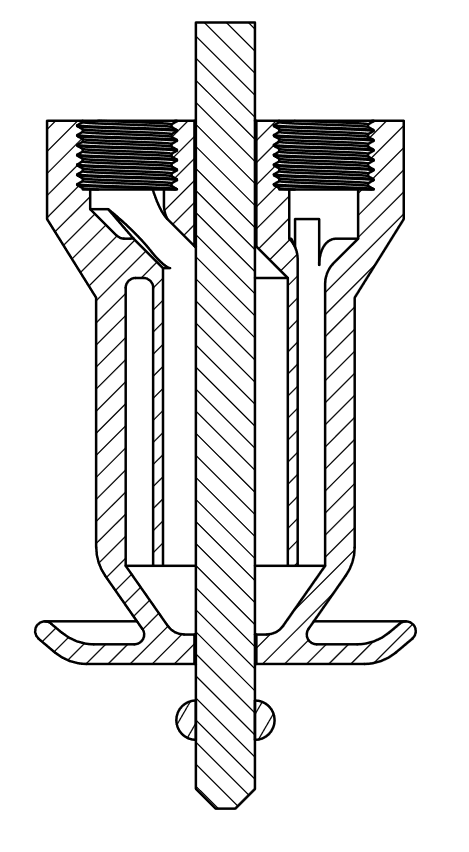
\includegraphics[height=7cm]{TempFinger}
	\caption{Querschnitt finger}
	\label{fig:querschnittfinger}
\end{figure}

The finger is also mounted on three stages and a track. This allows moving in all three axis and moving the finger out of the way with the track. Also the force for lifting is applied through the stages by manually moving the assembly up.

